\documentclass[xcolor=dvipsnames , 11pt]{beamer}
\mode<presentation>{}

\usepackage{Sweave}
\usepackage{booktabs}
\usepackage{float}
\usepackage[english]{babel}
\usepackage{tikz}
\usepackage{listings}
\usepackage{amsmath,amssymb}
%\usecolortheme{dove}
%\usecolortheme{rose}
\definecolor{links}{HTML}{2A1B81}
\hypersetup{colorlinks,linkcolor=,urlcolor=links}
\restylefloat{table}
%\usetheme{Frankfurt}
%\usetheme{Singapore}
\usetheme{CambridgeUS}
%\usetheme{Pittsburgh}
\usecolortheme[named=Blue]{structure}
\begin{document}
\Sconcordance{concordance:lesson_graphs_presentation.tex:lesson_graphs_presentation.Rnw:%
1 39 1 1 18 16 1 1 2 5 0 1 2 12 1 1 2 5 0 1 2 11 1 1 2 5 0 1 2 12 1 1 2 %
5 0 1 2 14 1 1 2 5 0 1 2 10 1 1 2 5 0 1 2 12 1 1 2 1 0 3 1 4 0 1 2 70 1}


% \usepackage{beamerthemesplit} // Activate for custom appearance

\title{\textbf{Graphical Exploration of Data \\
in R}}
% \date{\today}
\author{Mike Ooko}
\titlepage{}

\begin{frame}{\textbf{Why use graphics in data Analysis?}}

\begin{itemize}
\item{To understand data properties}
\item{To communucate results}
\end{itemize}
\end{frame}



\begin{frame}{\textbf{Graphs of single quantitative variables}}
\begin{itemize}
\item{\textbf{Box(-whisker)plot}}
\end{itemize}
It is suitable for skewed data, where it may not be correct to show mean and standard deviations.
\begin{figure}
\includegraphics[width=7.1cm, height=6cm]{box.png}
\end{figure}

\end{frame}

\begin{frame}[fragile]{\textbf{Boxplots}}
\setkeys{Gin}{width=0.62\linewidth}
\begin{center}
\begin{figure}
\centering
\begin{Schunk}
\begin{Sinput}
> boxplot(maltreat$weight)
\end{Sinput}
\end{Schunk}
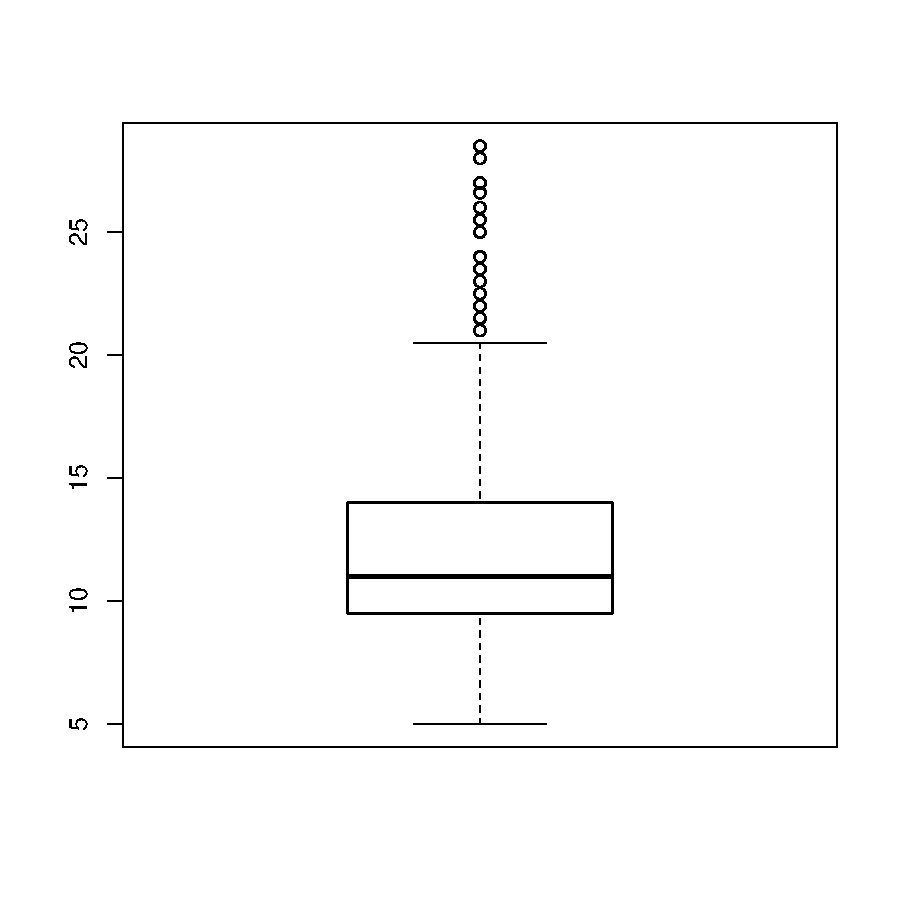
\includegraphics{lesson_graphs_presentation-002}

\end{figure}
\end{center}


\end{frame}


\begin{frame}[fragile]{\textbf{Boxplots}}
\setkeys{Gin}{width=0.6\linewidth}
\begin{center}
\begin{figure}
\centering
\begin{Schunk}
\begin{Sinput}
> boxplot(maltreat$weight~maltreat$sex,col="grey")
\end{Sinput}
\end{Schunk}
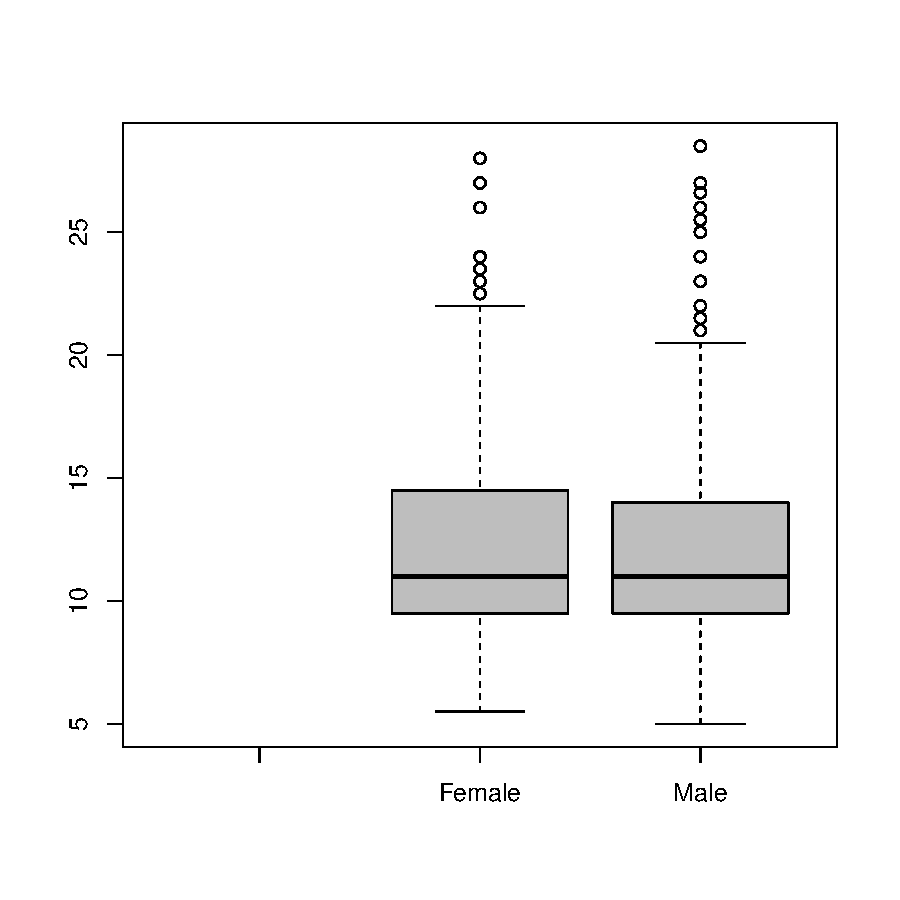
\includegraphics{lesson_graphs_presentation-003}
\end{figure}
\end{center}


\end{frame}

\begin{frame}[fragile]{\textbf{Histograms}}
Explore the assumption of normality.\vspace{0.4cm}
\setkeys{Gin}{width=0.6\linewidth}
\begin{center}
\begin{figure}
\centering
\begin{Schunk}
\begin{Sinput}
> hist(maltreat$weight, col="grey")
\end{Sinput}
\end{Schunk}
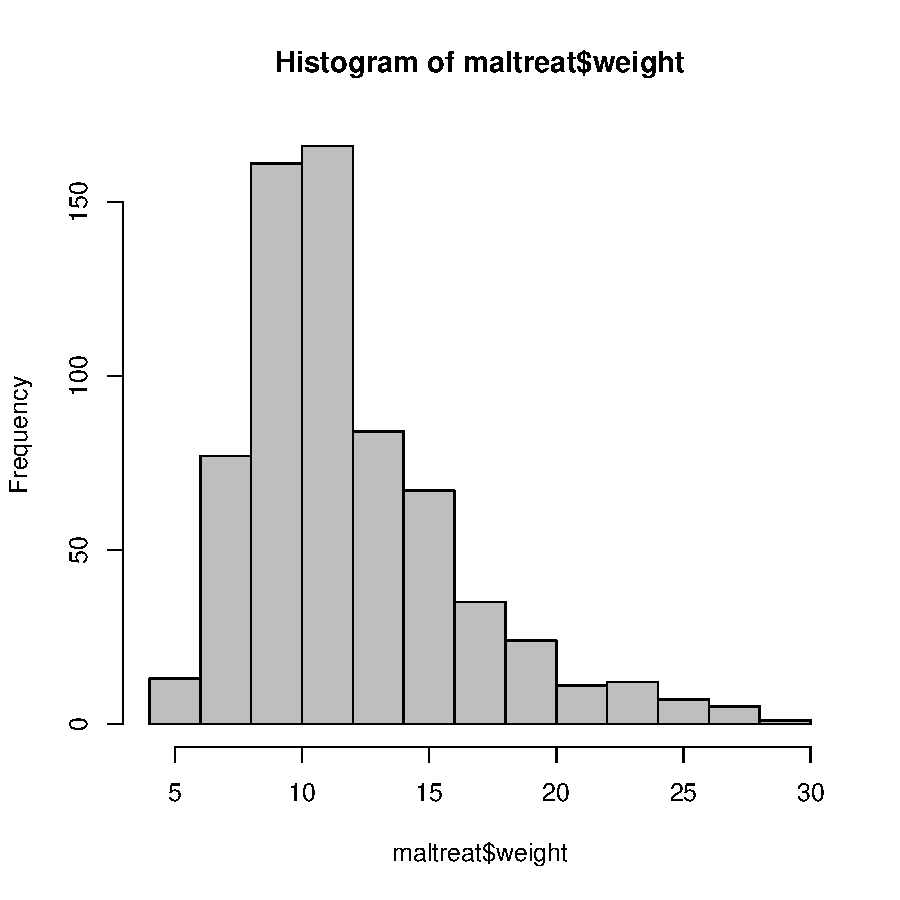
\includegraphics{lesson_graphs_presentation-004}
\end{figure}
\end{center}

\end{frame}

\begin{frame}[fragile]{\textbf{Scatterplots}}
\begin{itemize}
\item Visualize relationship between two quantitative variables.\vspace{0.3cm}
\end{itemize}
\setkeys{Gin}{width=0.5\linewidth}
\begin{center}
\begin{figure}
\centering
\begin{Schunk}
\begin{Sinput}
> plot(maltreat$weight,maltreat$falcsex, pch=19,col="blue")
\end{Sinput}
\end{Schunk}
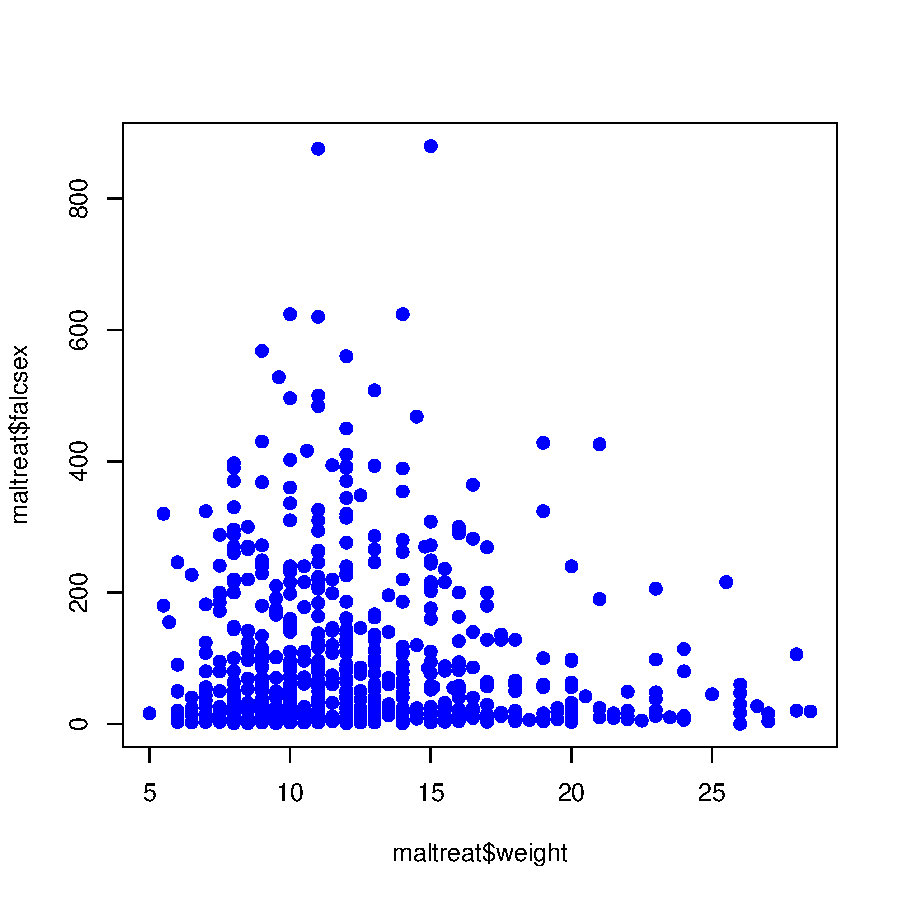
\includegraphics{lesson_graphs_presentation-005}
\end{figure}
\end{center}



\end{frame}

\begin{frame}[fragile]{\textbf{Graphs on single qualitative variables}}
\begin{itemize}
\item \textbf{Bar plots}
\end{itemize}
\setkeys{Gin}{width=0.6\linewidth}
\begin{center}
\begin{figure}
\centering
\begin{Schunk}
\begin{Sinput}
> barplot(table(maltreat$sex))
\end{Sinput}
\end{Schunk}
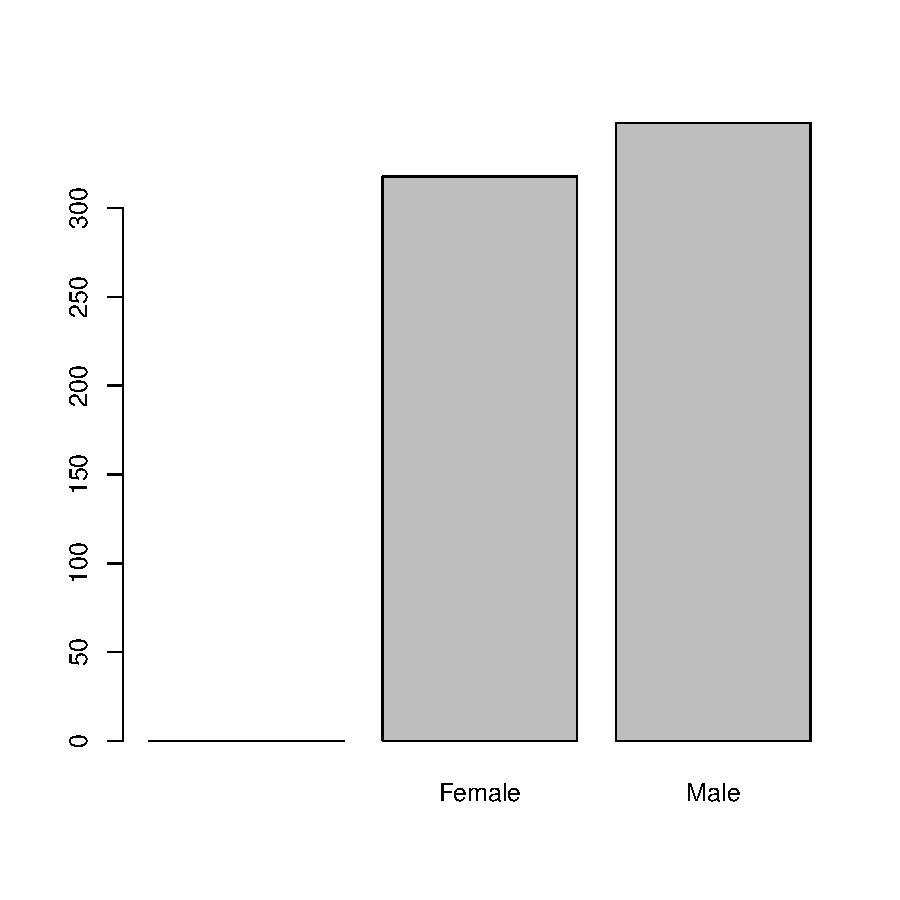
\includegraphics{lesson_graphs_presentation-006}
\end{figure}
\end{center}

\end{frame}

\begin{frame}[fragile]{\textbf{Pie charts}}

\setkeys{Gin}{width=0.62\linewidth}
\begin{center}
\begin{figure}
\centering
\begin{Schunk}
\begin{Sinput}
> pie(table(maltreat$sex), col=c("red","blue"),main="Pie chart of gender")
\end{Sinput}
\end{Schunk}
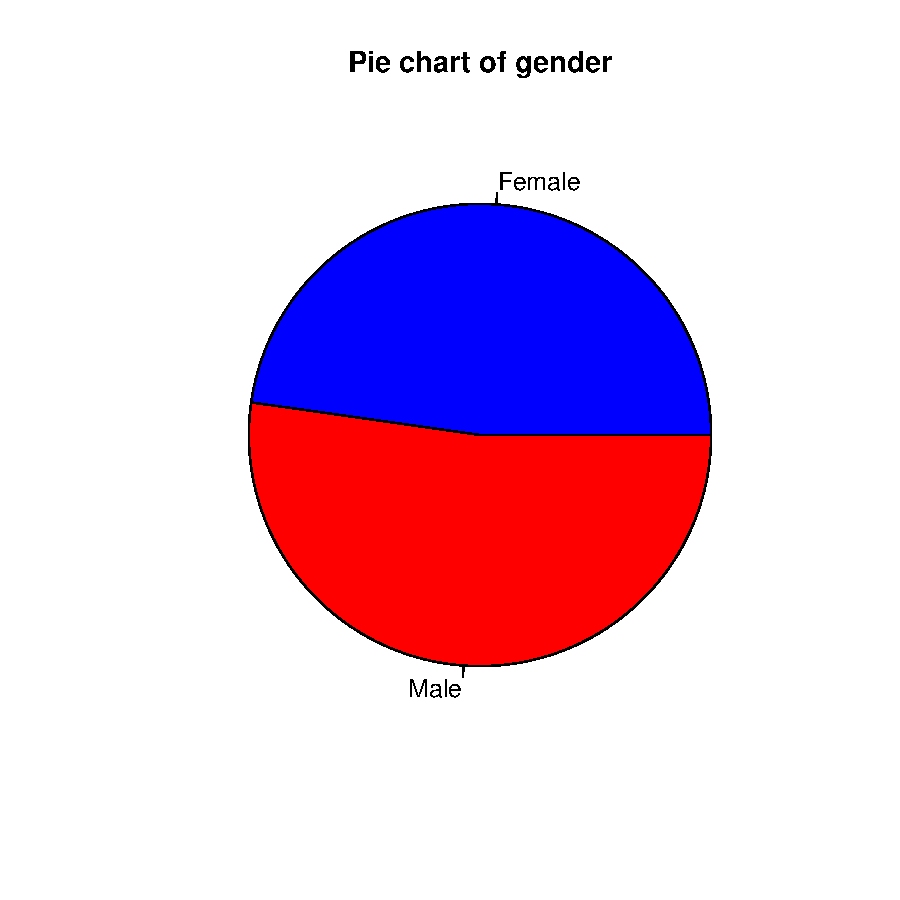
\includegraphics{lesson_graphs_presentation-007}
\end{figure}
\end{center}

\end{frame}



\begin{frame}[fragile]{\textbf{QQ Plots}}

\setkeys{Gin}{width=0.58\linewidth}
\begin{center}
\begin{figure}
\centering
\begin{Schunk}
\begin{Sinput}
> x<-rnorm(20)
> y<-rnorm(20)
> qqplot(x,y)
> abline(c(0,1))
\end{Sinput}
\end{Schunk}
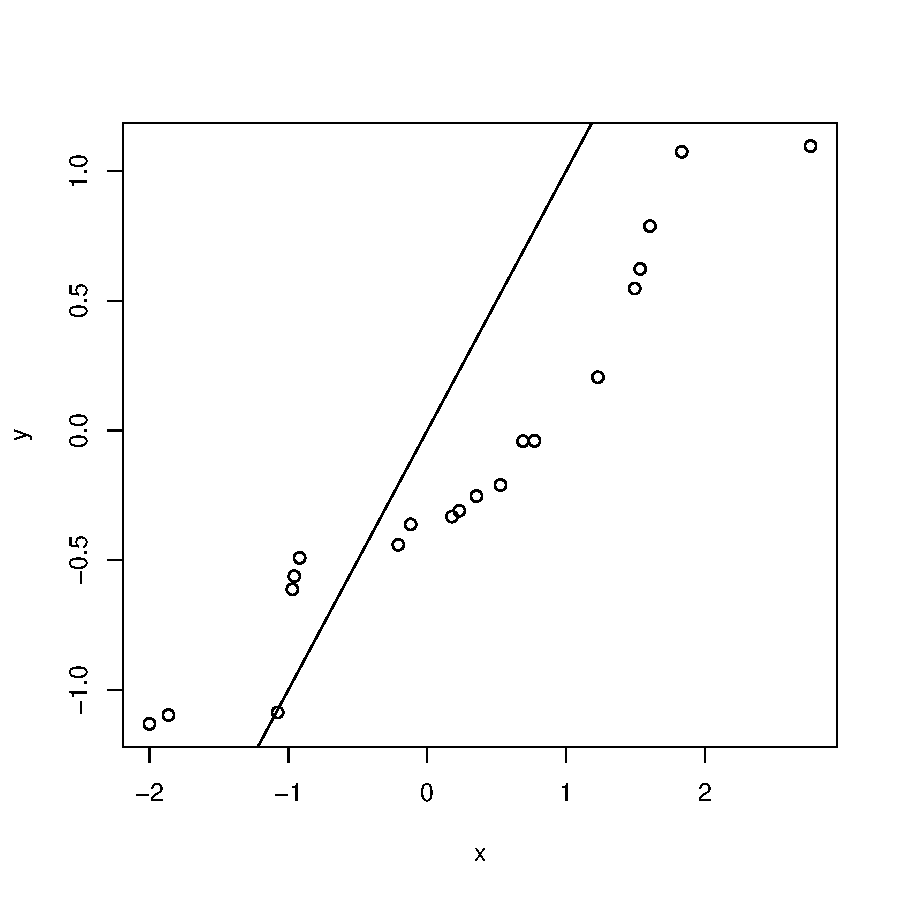
\includegraphics{lesson_graphs_presentation-008}
\end{figure}
\end{center}

\end{frame}

\begin{frame}{\textbf{Graphical workflow}}

\begin{itemize}
\begin{pause}
\item{Start with a rough plot}
\end{pause}
\begin{pause}
\item{Tweak it to make it expository}
\end{pause}
\begin{pause}
\item{Save the file}
\end{pause}
\begin{pause}
\item{Include it in presentations/manuscript}
\end{pause}
\end{itemize}
\end{frame}

\begin{frame}[fragile]{\textbf{Useful Graphical Parameters}}

\setkeys{Gin}{width=0.62\linewidth}
\textbf{par} function gives the parameters for the plot window.
\begin{itemize}
\item pch: the plotting symbol (default is open circle)
\item lty: the line type (default is solid line), can be dashed, dotted, etc.
\item lwd: the line width, specified as an integer multiple
\item col: the plotting color, specified as a number, string, or hex code; the colorsfunction gives you a vector of colors by name. colors() gives a list of all the available colours.
\item las: the orientation of the axis labels on the plot
\end{itemize}
\end{frame}

\begin{frame}[fragile]{\textbf{Useful Graphical Parameters}}

\setkeys{Gin}{width=0.62\linewidth}

\begin{itemize}
\item bg: the background color
\item mar: the margin size
\item mtext: add arbitrary text to the margins (inner or outer) of the plot
\item mfrow: number of plots per row, column (plots are filled row-wise)
\item mfcol: number of plots per row, column (plots are filled column-wise)
\end{itemize}
\end{frame}

\begin{frame}[fragile]{\textbf{Resources}}

\setkeys{Gin}{width=0.62\linewidth}

\href{http://rgraphgallery.blogspot.com/}{  R graph gallery} 

\href{http://www.cookbook-r.com/Graphs/}{  Cookbook for R}

\href{http://www.jstor.org/discover/10.2307/2683253?uid=3738336&uid=2&uid=4&sid=21103314330371}{  How to display data badly}






\end{frame}





\end{document}
